\selectlanguage{english}%

\chapter{Resultados} \label{capRes}

O modelo fuzzy desenvolvido a partir das seções anteriores foi simulado utilizando o software MATLAB \cite{matlab} e implementado na bancada real via CLP Rockwell. As seções a seguir apresentam os resultados obtidos em cada caso.

\section{Simulações} \label{secAnalise}
A planta de quatro-tanques, como apresentada no \jhhref{capDescSis}{capítulo}, compõe um sistema capaz de ilustrar diversas dinâmicas para suas variáveis de processo. Assim, são escolhidas uma configuração em \textbf{fase mínima }e outra em \textbf{fase não-mínima} e a partir delas a modelagem e o controlador fuzzy são desenvolvidos. 

\subsection{Fase Mínima}
Nesta configuração a maior parte do fluído que saí das bombas é direcionado diretamente para os tanques controlados, ou seja $\gamma_i > 0.5$. A \jhhref{tabFaseMinima}{tablea} a seguir apresenta suas especificações.

\begin{center} \label{tabFaseMinima}
	\begin{tabular}{|c|c|}
		\hline
		\multicolumn{2}{|c|}{Especificações Iniciais da Planta} \\
		\hline
		A1, A3 $(cm^2)$ & 28 \\ \hline
		A2, A4 $(cm^2)$ & 32 \\ \hline
		a1, a3 $(cm^2)$ & 0.071 \\ \hline
		a2, a4 $(cm^2)$ & 0.057 \\ \hline
		g $cm/s$ & 981 \\ \hline
		k1 & 3,33 \\ \hline
		k2 & 3.35 \\ \hline
		$\gamma_1$ & 0.70 \\ \hline
		$\gamma_2$ & 0.60 \\ \hline
		\hline
	\end{tabular}
\end{center}

O \jhhref{eqModNL}{modelo não linear} para esta configuração é:
\begin{equation}
\begin{cases}
\dot{h_{1}} = \frac{1}{A_{1}}(a_{3}\sqrt{2gh_{3}} + \gamma_{1}k_{1}v_{1} - a_{1}\sqrt{2gh_{1}})\\

\dot{h_{2}} = \frac{1}{A_{2}}(a_{4}\sqrt{2gh_{4}} + \gamma_{2}k_{2}v_{2} - a_{2}\sqrt{2gh_{2}})\\

\dot{h_{3}} = \frac{1}{A_{3}}((1 - \gamma_{2})k_{2}v_{2} - a_{3}\sqrt{2gh_{3}})\\

\dot{h_{4}} = \frac{1}{A_{4}}((1 - \gamma_{1})k_{1}v_{1} - a_{4}\sqrt{2gh_{4}})
\end{cases}
\label{eqFMNL}
\end{equation}

Escolhendo os cojuntos fuzzy \{"baixo","alto"\} e definindo \{5 , 15\} como seus representantes os níveis 1 e 2, por combinação simples obtém-se os seguintes pontos de linearização:
\begin{center}
	\begin{tabular}{|c|c|c|c|c|c|c|}
		\hline
		Sistema & Nível 1 ($\bar{h_1}$) & Nível 2 ($\bar{h_2}$) & Nível 3 ($\bar{h_3}$) & Nível 1 ($\bar{h_4}$) & Tensão 1 ($\bar{v_1}$) & Tensão 2 ($\bar{v_2}$) \\ \hline
		1 & 5 & 5 & 10 & 10 & 10 & 10 \\ \hline
		2 & 5 & 15 & 10 & 10 & 10 & 10 \\ \hline
		3 & 15 & 5 & 10 & 10 & 10 & 10 \\ \hline
		4 & 15 & 15 & 10 & 10 & 10 & 10 \\	\hline
	\end{tabular}
\end{center}

Haverá então quatro regras Se-Então para composição do modelo TS final. As imagens a seguir apresenta a comparação entre os modelos \jhhref{eqModNL}{não-linear}, \jhhref{eqModLinear}{linearizado} em um ponto único e \jhhref{eqTakSugPlanta}{Takagi-Sugeno}:

\begin{figure}[H]
	\centering
	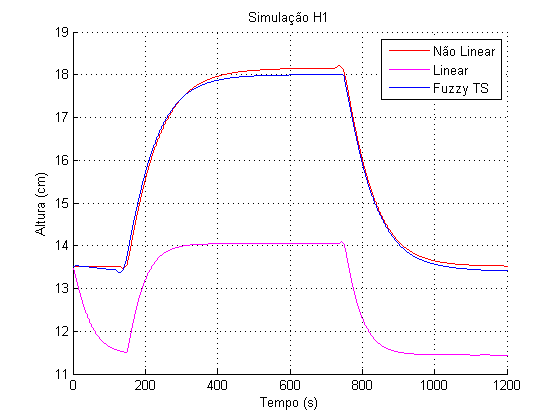
\includegraphics[width=0.7\textwidth]{img/FM_h1_5_10_15.png}
	\caption{\small Linearização Convencional: $ \bar{h1}=5, \bar{h2}=5$. Linearizações Fuzzy: $\bar{h1}=[10 \ \ 15] \ \ \bar{h2}=[10 \ \ 15]$ }
	\label{figH1TS2}
\end{figure}

\begin{figure}[H]
	\centering
	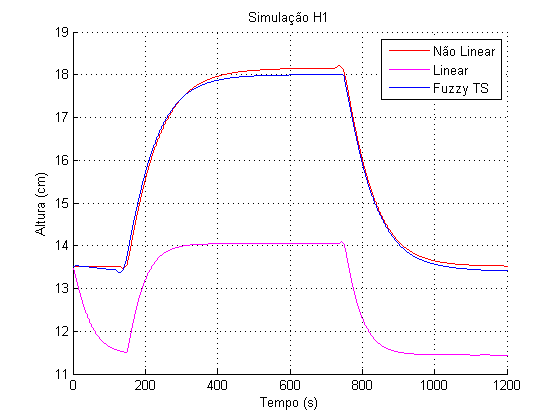
\includegraphics[width=0.7\textwidth]{img/FM_h1_5_10_15.png}
	\caption{\small Linearização Convencional: $ \bar{h1}=5, \bar{h2}=5$. Linearizações Fuzzy: $\bar{h1}=[10 \ \ 15] \ \ \bar{h2}=[10 \ \ 15]$ }
	\label{figH2TS2}
\end{figure}

É notável que o modelo fuzzy representa de modo mais eficiente o sistema. Como dito, o modelo TS pode se aproximar o quanto se desejar do não-linear no qual se baseia. A \jhhref{imgTS5}{imagem} apresenta um modelo com 5 conjuntos para os dois níveis e a \jhhref{imgTS15}{imagem} utilizando 15. É importante notar, no entanto, que a complexidade do modelo é exponencial, devido a combinação dos conjuntos das variáveis linguísticas presentes, assim, o primeiro é composto por 25 regras Se-Então e o segundo por 225!

\begin{figure}[H]
	\centering
	\begin{tabular}{cc}
		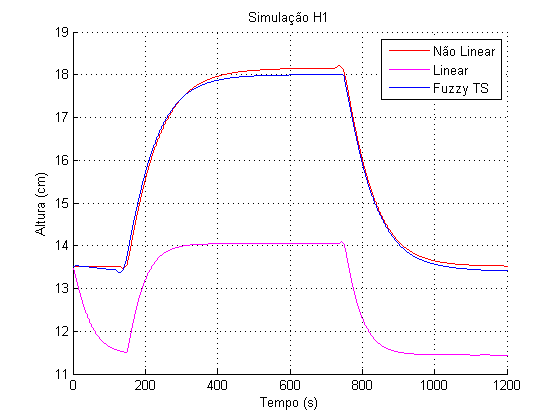
\includegraphics[width=0.5\textwidth,keepaspectratio]{img/FM_h1_5_10_15.png} &
		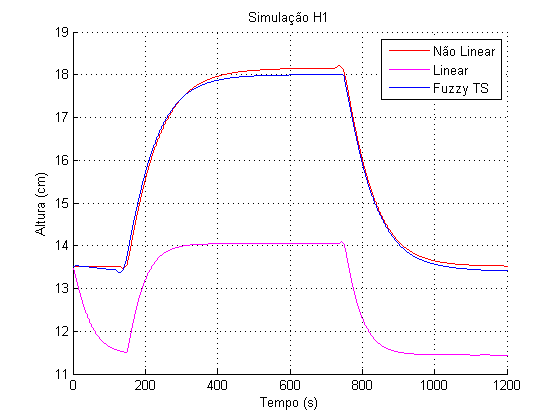
\includegraphics[width=0.5\textwidth,keepaspectratio]{img/FM_h1_5_10_15.png} \\
		(a) Pertinência do conjunto "muito frio" &
		(b) Pertinência do conjunto "frio"
	\end{tabular}
	\caption{\label{imgTS5} Funções de Pertinência.}
\end{figure}

\begin{figure}[H]
	\centering
	\begin{tabular}{cc}
		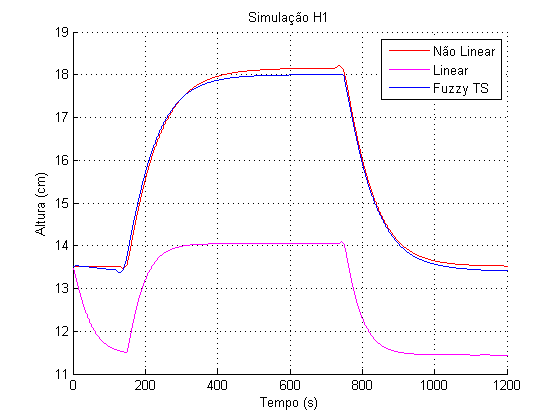
\includegraphics[width=0.5\textwidth,keepaspectratio]{img/FM_h1_5_10_15.png} &
		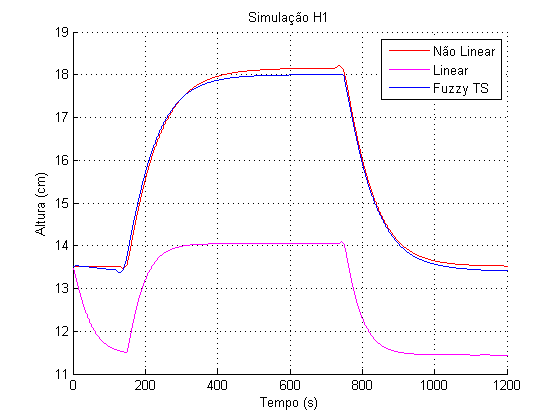
\includegraphics[width=0.5\textwidth,keepaspectratio]{img/FM_h1_5_10_15.png} \\
		(a) Pertinência do conjunto "muito frio" &
		(b) Pertinência do conjunto "frio"
	\end{tabular}
	\caption{\label{imgTS15} Funções de Pertinência.}
\end{figure}

A partir das \jhhref{eqContFuzzy}{equações} são desenvolvidos os controladores para cada uma das regras. A tabela a seguir apresenta os ganhos obtidos:
\begin{center}
	\begin{tabular}{|c|c|}
		\hline
		Regra & Ganho \\ \hline
		 1 & $ K = 
			\begin{bmatrix}
				1 & 2 & 3 & 4 & 5 & 6 \\
				1 & 2 & 3 & 4 & 5 & 6
			\end{bmatrix}$ \\[20pt] \hline
		2 & $ K = 
			\begin{bmatrix}
				1 & 2 & 3 & 4 & 5 & 6 \\
				1 & 2 & 3 & 4 & 5 & 6
			\end{bmatrix}$ \\[20pt] \hline
		3 & $ K = 
			\begin{bmatrix}
				1 & 2 & 3 & 4 & 5 & 6 \\
				1 & 2 & 3 & 4 & 5 & 6
			\end{bmatrix}$ \\[20pt] \hline
		4 & $ K = 
			\begin{bmatrix}
				1 & 2 & 3 & 4 & 5 & 6 \\
				1 & 2 & 3 & 4 & 5 & 6
			\end{bmatrix}$ \\[20pt] \hline
	\end{tabular}
\end{center}

\subsection{Fase Não-Mínima}
A tabela a seguir apresenta as especificações do sistema, nota-se por $\gamma_1$ e $\gamma_2$ que o sistema está em fase não mínima.
\begin{center}
	\begin{tabular}{|c|c|}
		\hline
		\multicolumn{2}{|c|}{Especificações do sistema} \\
		\hline'
		A1, A3 $(cm^2)$ & 28 \\ \hline
		A2, A4 $(cm^2)$ & 32 \\ \hline
		a1, a3 $(cm^2)$ & 0.071 \\ \hline
		a2, a4 $(cm^2)$ & 0.057 \\ \hline
		g $(cm/s)$ & 981 \\ \hline
		k1 & 3,14 \\ \hline
		k2 & 3.29 \\ \hline
		$\gamma_1$ & 0.43 \\ \hline
		$\gamma_2$ & 0.34 \\ \hline
		\hline
	\end{tabular}
\end{center}

O \jhhref{eqModNL}{modelo não linear} para esta configuração é:
\begin{equation}
\begin{cases}
	\dot{h_{1}} = \frac{1}{A_{1}}(a_{3}\sqrt{2gh_{3}} + \gamma_{1}k_{1}v_{1} - a_{1}\sqrt{2gh_{1}})\\
	
	\dot{h_{2}} = \frac{1}{A_{2}}(a_{4}\sqrt{2gh_{4}} + \gamma_{2}k_{2}v_{2} - a_{2}\sqrt{2gh_{2}})\\
	
	\dot{h_{3}} = \frac{1}{A_{3}}((1 - \gamma_{2})k_{2}v_{2} - a_{3}\sqrt{2gh_{3}})\\
	
	\dot{h_{4}} = \frac{1}{A_{4}}((1 - \gamma_{1})k_{1}v_{1} - a_{4}\sqrt{2gh_{4}})
\end{cases}
\label{eqFNMNL}
\end{equation}

Escolhendo os cojuntos fuzzy \{"baixo","alto"\} e definindo {5,15} para os níveis 1 e 2, obtém-se, a partir da\jhhref{eqFMNL}{equação} os seguintes pontos de linearização:

\begin{center}
	\begin{tabular}{|c|c|c|c|c|c|c|}
		\hline
		Sistema & Nível 1 ($h_1$) & Nível 2 ($h_2$) & Nível 3 ($h_3$) & Nível 1 ($h_4$) & Tensão 1 ($v_1$) & Tensão 2 ($v_2$) \\ \hline
		1 & 5 & 5 & 10 & 10 & 10 & 10 \\ \hline
		2 & 5 & 15 & 10 & 10 & 10 & 10 \\ \hline
		3 & 15 & 5 & 10 & 10 & 10 & 10 \\ \hline
		4 & 15 & 15 & 10 & 10 & 10 & 10 \\	\hline
	\end{tabular}
\end{center}

Nas figuras que se seguem apresentam-se as respostas dos modelos à degraus aplicados ao sistema.  Observa-se que o modelo linear apresenta bons resultados quando o estado do sistema é próximo ao ponto de operação. Já para os modelos fuzzy, quanto mais pontos de linearização utilizados, melhor o resultado, embora mais complexo o custo computacional.

\begin{figure}[H]
	\centering
	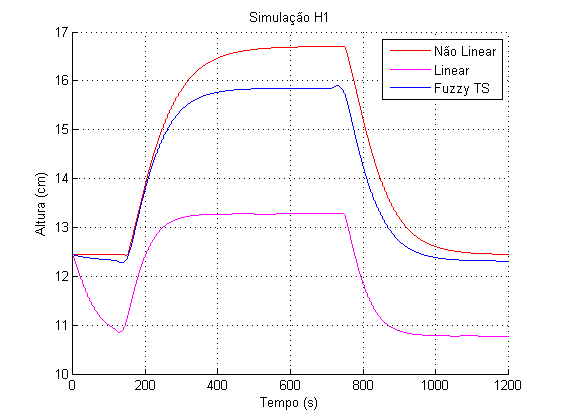
\includegraphics[width=0.7\textwidth]{img/h1Fuz5_10.png}
	\caption{\small Linearização Convencional: $ \bar{h1}=5, \bar{h2}=5$. Linearizações Fuzzy: $\bar{h1}=[5 \ \ 10] \ \ \bar{h2}=[5 \ \ 10]$ }
	\label{figH1FNM_1}
\end{figure}


\section{Implementação}

\selectlanguage{brazil}%

